% ———————————————————————————————————————————————————————————————————————————— %
%                                 Configuration                                %
% ———————————————————————————————————————————————————————————————————————————— %
\documentclass[conference, a4paper]{IEEEtran}
\IEEEoverridecommandlockouts
\usepackage{soul}
\usepackage{paralist}
\usepackage[utf8]{inputenc}
\newtheorem{theorem}{Teorema}
\usepackage{cite}
\usepackage{amsmath, amssymb, amsfonts}
\usepackage{textcomp}
\usepackage{url}
\usepackage[table]{xcolor}
\usepackage{xcolor}
\usepackage{float}
\usepackage{enumitem}
\usepackage{acro}
\usepackage{multicol}
\usepackage{mathtools}
\usepackage{longtable}
\usepackage{diagbox, hhline, booktabs}
\usepackage{multirow}
\usepackage{graphicx}
\usepackage{booktabs}
\usepackage{makecell}
\usepackage{siunitx}
\usepackage{changepage}
\usepackage{algorithm}
\usepackage{algpseudocode}
\usepackage{balance}
\usepackage{float}

% ———————————————————— For using tikz code as image input ———————————————————— %
\usepackage{tikz}
\usepackage{pgfplots}
\usepackage[dvipsnames]{xcolor}
\usepgfplotslibrary{groupplots}
\pgfplotsset{compat=1.18}
\usepackage[caption=false, font=normalsize, labelfont=sf, textfont=sf]{subfig}
\usepackage{xurl}

% ——————————————————————————— Hyperlinks and boxes ——————————————————————————— %
% Default, only shown at editor:
% \usepackage{{hyperref}}

% Blue Text:
% \usepackage[colorlinks=true, linkcolor=black, citecolor=blue, urlcolor=blue]{
%   hyperref
% }
\usepackage{hyperref}

% Boxes:
\setlength{\fboxsep}{1pt}
\setlength{\fboxrule}{1pt}
\newcommand{\refbox}[1]{%
\fcolorbox{blue}{white}{\ref{#1}}%
}
\newcommand{\eqbox}[1]{\ensuremath{%
\fcolorbox{blue}{white}{(\ref{#1})}%
}}
% ———————————————————————————————————————————————————————————————————————————— %
% centered math for numbers
\newcolumntype{N}{>{$}c<{$}} 

% Primeiro uso: "Longo (Curto, do inglês Foreign)"
% \RenewAcroTemplate{long-short}{%
%   \acrowrite{long}\acspace
%   (%
%     \acrowrite{short}%
%     \acroifT{foreign}{, do inglês \acrowrite{foreign}}%
%   )%
% }

\renewcommand{\theequation}{\arabic{equation}}

% ———————————————————————————————————————————————————————————————————————————— %
\usepackage{scalerel}
\usepackage{tikz}
\usetikzlibrary{svg.path}
\definecolor{orcidlogocol}{HTML}{A6CE39}
\tikzset{
  orcidlogo/.pic={
    \fill[orcidlogocol] svg{M256,128c0,70.7-57.3,128-128,128C57.3,256,0,198.7,0,128C0,57.3,57.3,0,128,0C198.7,0,256,57.3,256,128z};
    \fill[white] svg{M86.3,186.2H70.9V79.1h15.4v48.4V186.2z}
                 svg{M108.9,79.1h41.6c39.6,0,57,28.3,57,53.6c0,27.5-21.5,53.6-56.8,53.6h-41.8V79.1z M124.3,172.4h24.5c34.9,0,42.9-26.5,42.9-39.7c0-21.5-13.7-39.7-43.7-39.7h-23.7V172.4z}
                 svg{M88.7,56.8c0,5.5-4.5,10.1-10.1,10.1c-5.6,0-10.1-4.6-10.1-10.1c0-5.6,4.5-10.1,10.1-10.1C84.2,46.7,88.7,51.3,88.7,56.8z};
  }
}

\newcommand\orcid[1]{\href{https://orcid.org/#1}{\mbox{\scalerel*{

\begin{tikzpicture}[yscale=-1,transform shape]
\pic{orcidlogo};
\end{tikzpicture}
}{|}}}}

% ———————————————————————————————————————————————————————————————————————————— %
\renewcommand{\citeleft}{[}
\renewcommand{\citeright}{]}
\renewcommand{\citemid}{, }
\renewcommand{\citepunct}{, }
\renewcommand{\citedash}{-} % Packages are located in this file
\DeclareAcronym{BS}{
  short = BS,
  long = base station,
  long-plural-form = base stations
} % Acronyms are located in this file
\begin{document}
\title{Title}
\author{
\IEEEauthorblockN{
  Matheus F. Silva\orcid{0009-0003-3374-3572}\IEEEauthorrefmark{1},
  Felipe A. P. de Figueiredo\orcid{0000-0002-2167-7286}\IEEEauthorrefmark{1}
  \IEEEauthorblockA{
    \IEEEauthorrefmark{1}National Institute of Telecommunications, Inatel, Santa Rita do Sapuca\'i, MG, Brazil. \\
    Email: \{matheus.f, felipe.figueiredo\}@inatel.br
    }
  %\thanks{}
  }
}

\maketitle % Authors and thanks text

% ———————————————————————————————————————————————————————————————————————————— %
%                                   Abstract                                   %
% ———————————————————————————————————————————————————————————————————————————— %
\begin{abstract}
Your abstract should provide a summary of the research conducted, the conclusions reached, and the potential implications of those conclusions. A strong abstract will also: Consist of a single paragraph up to 250 words, with correct grammar and unambiguous terminology Be self-contained; without abbreviations, footnotes, references, or mathematical equations Highlight what is novel in your work Include 3-5 keywords or phrases that describe the research, with any abbreviations clearly defined, to help readers find your article Most authors write the abstract last and edit it multiple times before article publication to ensure it accurately captures the entire article. IEEE recommends that you do not include mathematical symbols in your article title or abstract because they may not display properly.

\end{abstract}

\begin{IEEEkeywords}
TODO.
\end{IEEEkeywords}

\acresetall


% ———————————————————————————————————————————————————————————————————————————— %
%                                 Introduction                                 %
% ———————————————————————————————————————————————————————————————————————————— %
\section{Introduction}
\label{introduction}

Read \cite{ieee_author_center_structure_article_2025}.

% ———————————————————————————————————————————————————————————————————————————— %
%                                   Section 1                                  %
% ———————————————————————————————————————————————————————————————————————————— %
\section{Section 1}
\label{s1}

Examples of images:

% One column
\begin{figure}[httb]
\centering
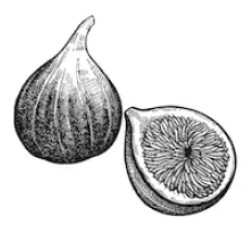
\includegraphics[width=2.5in]{figures/example.png}
\caption{TODO.}
\label{fig_1}
\end{figure}

% Two columns
\begin{figure*}[httb]
\centering
\subfloat[]{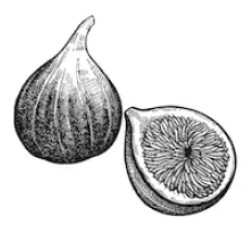
\includegraphics[width=2.5in]{figures/example.png}%
\label{fig_first_case}} \hfil \subfloat[]{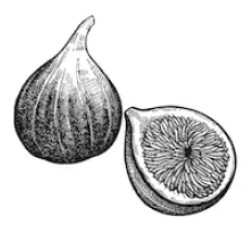
\includegraphics[width=2.5in]{figures/example.png}%
\label{fig_second_case}}
\caption{TODO. (a) Case I. (b) Case II.}
\label{fig_sim}
\end{figure*}

% Tikz input example:
\begin{figure*}[httb]
\centering
\input{figures/tikz/example-csv.tikz}
\caption{TODO.}
\label{fig:results}
\end{figure*}

% ———————————————————————————————————————————————————————————————————————————— %
%                                   Section 2                                  %
% ———————————————————————————————————————————————————————————————————————————— %

\section{Float placement in \LaTeX}
\label{sec:float-placement}

This section summarizes all figure and table placement specifiers and
practical usage.

\subsection*{Specifiers}
\begin{table}[t]
\centering
\begin{tabular}{ll}
\hline
Specifier  & Meaning                                                          \\
\hline
\texttt{h} & Place here if space allows                                       \\
\texttt{t} & Place at top of page or column                                   \\
\texttt{b} & Place at bottom of page or column                                \\
\texttt{p} & Place on a float-only page                                       \\
\texttt{!} & Relax placement constraints for this float                       \\
\texttt{H} & Exact here, requires \texttt{\textbackslash usepackage\{float\}} \\
\hline
\end{tabular}
\end{table}

\subsection*{Combination rules and defaults}
\begin{itemize}
\item Combine letters to declare allowed targets, for example \texttt{[ht]},
\texttt{[tbp]}, \texttt{[!htbp]}. Order does not matter; duplicates are ignored.

\item Default for \texttt{figure} and \texttt{table} is \texttt{[tbp]}.

\item In two-column mode, \texttt{figure*} and \texttt{table*} default to
\texttt{[tp]} only.
\end{itemize}

\subsection*{Two-column specifics}
\begin{itemize}
\item Bottom placement of full-width floats is disabled by default. To allow
it, load \texttt{dblfloatfix} or \texttt{stfloats}. Then \texttt{[tbp]} works
for \texttt{figure*} and \texttt{table*}.
\end{itemize}

\subsection*{Practical guidance}
\begin{itemize}
\item Avoid using only \texttt{[h]}. Prefer \texttt{[!htbp]} for robust
placement.

\item Allowing \texttt{t} lets floats move earlier on the page. If that is undesirable,
consider \texttt{\textbackslash suppressfloats[t]} or the \texttt{flafter}
package.

\item \texttt{[H]} forces exact placement and disables floating. Use sparingly,
and only with the \texttt{float} package.
\end{itemize}

\subsection*{Drop-in settings for this manuscript}
Single column: \begin{verbatim}
\begin{figure}[!htbp]
\centering
% ...
\end{figure}
\end{verbatim}

Two columns, default:
\begin{verbatim}
\begin{figure*}[t]
\centering
% ...
\end{figure*}
\end{verbatim}

\section*{Acknowledgments}
This should be a simple paragraph before the References to thank those individuals and institutions who have supported your work on this article.

% ———————————————————————————————————————————————————————————————————————————— %
%                                  References                                  %
% ———————————————————————————————————————————————————————————————————————————— %

% USE "and others" for papers with more than 2 authors.
\bibliographystyle{IEEEtran}
\bibliography{IEEEabrv,references}

% ———————————————————————————————————————————————————————————————————————————— %
%                                   Biography                                  %
% ———————————————————————————————————————————————————————————————————————————— %

\begin{IEEEbiography}
[{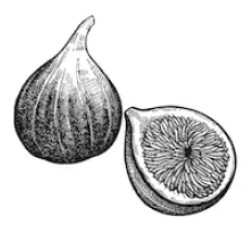
\includegraphics[width=1in,height=1.25in,clip,keepaspectratio]{figures/example.png}}]{Michael Shell}
Use $\backslash${\tt{begin\{IEEEbiography\}}} and then for the 1st argument use
$\backslash${\tt{includegraphics}} to declare and link the author photo. Use
the author name as the 3rd argument, followed by the biography text.
\end{IEEEbiography}

\bf{If you will not include a photo:}
\begin{IEEEbiographynophoto}
{John Doe} Use $\backslash${\tt{begin\{IEEEbiographynophoto\}}} and the
author name as the argument, followed by the biography text.
\end{IEEEbiographynophoto}

% ———————————————————————————————————————————————————————————————————————————— %
\end{document}